\section{Actividades}
Realizar las actividades solicitadas, en ellas se realizará la comunicación serie asíncrona, será empleada el formato REPL usando la interfaz por default; así como las siguientes interfaces.

\subsection{Ejercicio 1}
Escribir el siguiente programa:

\begin{lstlisting}
import select
import sys
import time
import machine

poll_obj = select.poll()
poll_obj.register(sys.stdin, 1)
sys.stdout.write("Esperando recepción de datos \n")
print("Tecla un carácter y luego <enter>")
while True:
    if poll_obj.poll(0):
        ch = sys.stdin.read(1)
        sys.stdout.write("Dato recibido \n")
        print("Hola UNAM")
        time.sleep(0.1)
\end{lstlisting}

\begin{itemize}
    \item [a] Comentar el código.
    \item [b] Indicar que hace.
    \item [c] Ejecutar.
    \item [d] Ingresar datos desde la consola de Thonny.
    \item [e] Explicar la diferencia entre:
    \begin{itemize}
        \item [a] \texttt{sys.stdout.write("Esperando recepción de datos \textbackslash n")}
        \item [b] \texttt{print("Teclea un caracter y luego <enter>")}
\end{itemize}
\end{itemize}

\subsubsection{Pseudo Código}

\begin{algorithm}[H]
\SetAlgoLined
\caption{Lectura de datos desde entrada estándar}

Inicializar sistema de lectura no bloqueante\;
Registrar entrada estándar\;

Mostrar "Esperando recepción de datos"\;
Mostrar "Tecla un carácter y luego <enter>"\;

Mientras verdadero hacer\;
\Indp
    Verificar si hay datos disponibles en la entrada\;
    
    \If{hay datos disponibles}{
        Leer un carácter\;
        Mostrar "Dato recibido"\;
        Mostrar "Hola UNAM"\;
        Esperar 0.1 segundos\;
    }
\Indm

\end{algorithm}

\subsubsection{Desarrollo}
\begin{lstlisting}
import select
import sys
import time
import machine

# Crea un objeto 'poll' para realizar un seguimiento de eventos de entrada
poll_obj = select.poll()

# Registra la entrada estándar (teclado/consola) en el objeto poll
# El valor '1' indica que queremos monitorear el evento POLLIN (datos listos para leer)
poll_obj.register(sys.stdin, 1)

# Envía un mensaje a la consola indicando que el programa está listo
sys.stdout.write("Esperando recepción de datos \n")
print("Teclea un carácter y luego <enter>")

while True:
    # Verifica si hay datos disponibles en los objetos registrados (timeout de 0ms)
    # Si poll(0) devuelve una lista con contenido, significa que hay datos esperando
    if poll_obj.poll(0):
        # Lee un solo carácter de la entrada estándar
        ch = sys.stdin.read(1)
        
        # Confirma la recepción del dato
        sys.stdout.write("Dato recibido \n")
        
        # Imprime un saludo 
        print("Hola UNAM")
    
    time.sleep(0.1)
\end{lstlisting}

\newpage
\begin{figure}[ht!]
    \centering
    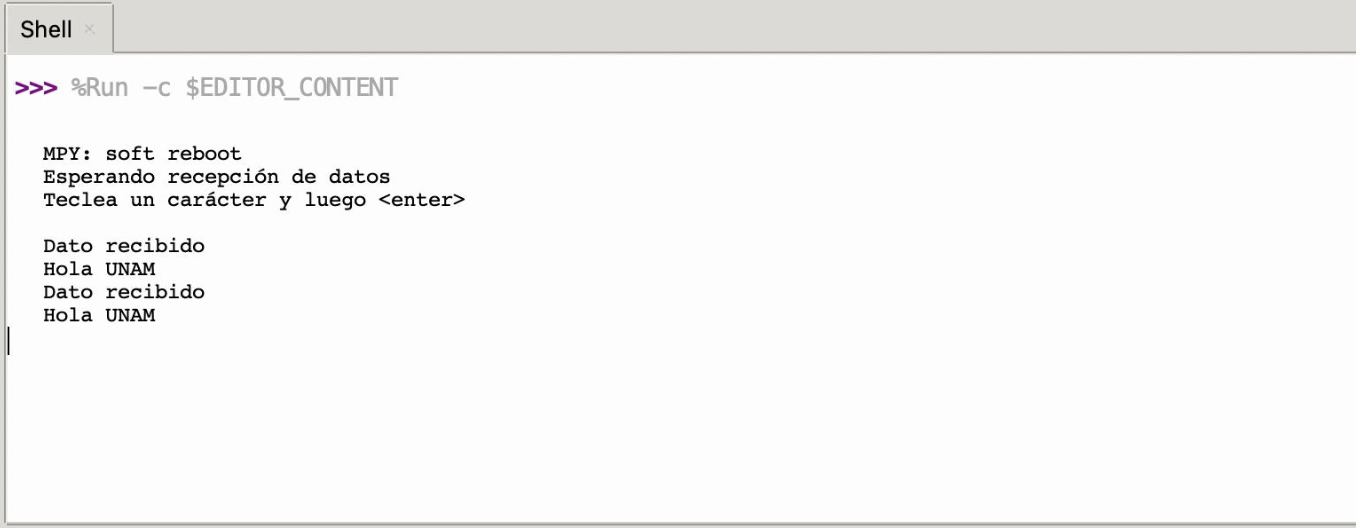
\includegraphics[width=\linewidth]{img/1.png}
    \caption*{Ejecución Ejercicio 1}
\end{figure}

\subsubsection{Análisis de resultados}
El programa funcionó correctamente al implementar una lectura no bloqueante de la entrada estándar mediante el uso de \texttt{poll()}, lo que permitió detectar cuando el usuario ingresaba datos sin detener la ejecución del ciclo principal. Se comprobó que cada vez que se presionaba una tecla seguida de \textit{enter}, el sistema respondía mostrando los mensajes ``Dato recibido'' y ``Hola UNAM''. Además, el uso de un retardo ayudó a evitar lecturas repetidas excesivas, manteniendo un comportamiento estable en la comunicación serial dentro del entorno REPL.


\newpage
%%%%%%%%%%%%%%%%%%%%%%%%%%%%%%%%%%%%%%%%%%%
\subsection{Ejercicio 2}

Para este ejercicio, realizar los pasos siguientes:

\begin{enumerate}[label=\alph*.]
    \item Ubicar el COM de conexión de la Raspberry Pi.
    \begin{figure}[ht!]
        \centering
        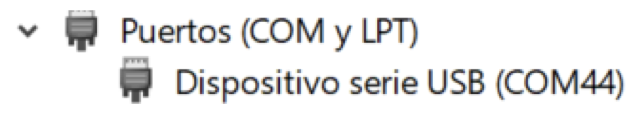
\includegraphics[width=0.4\linewidth]{pics/2-1.png}
        \caption*{Figura 7-4. Información del Administrador de Dispositivos}
    \end{figure}

    \item Abrir la terminal de su preferencia.
    \begin{figure}[ht!]
        \centering
        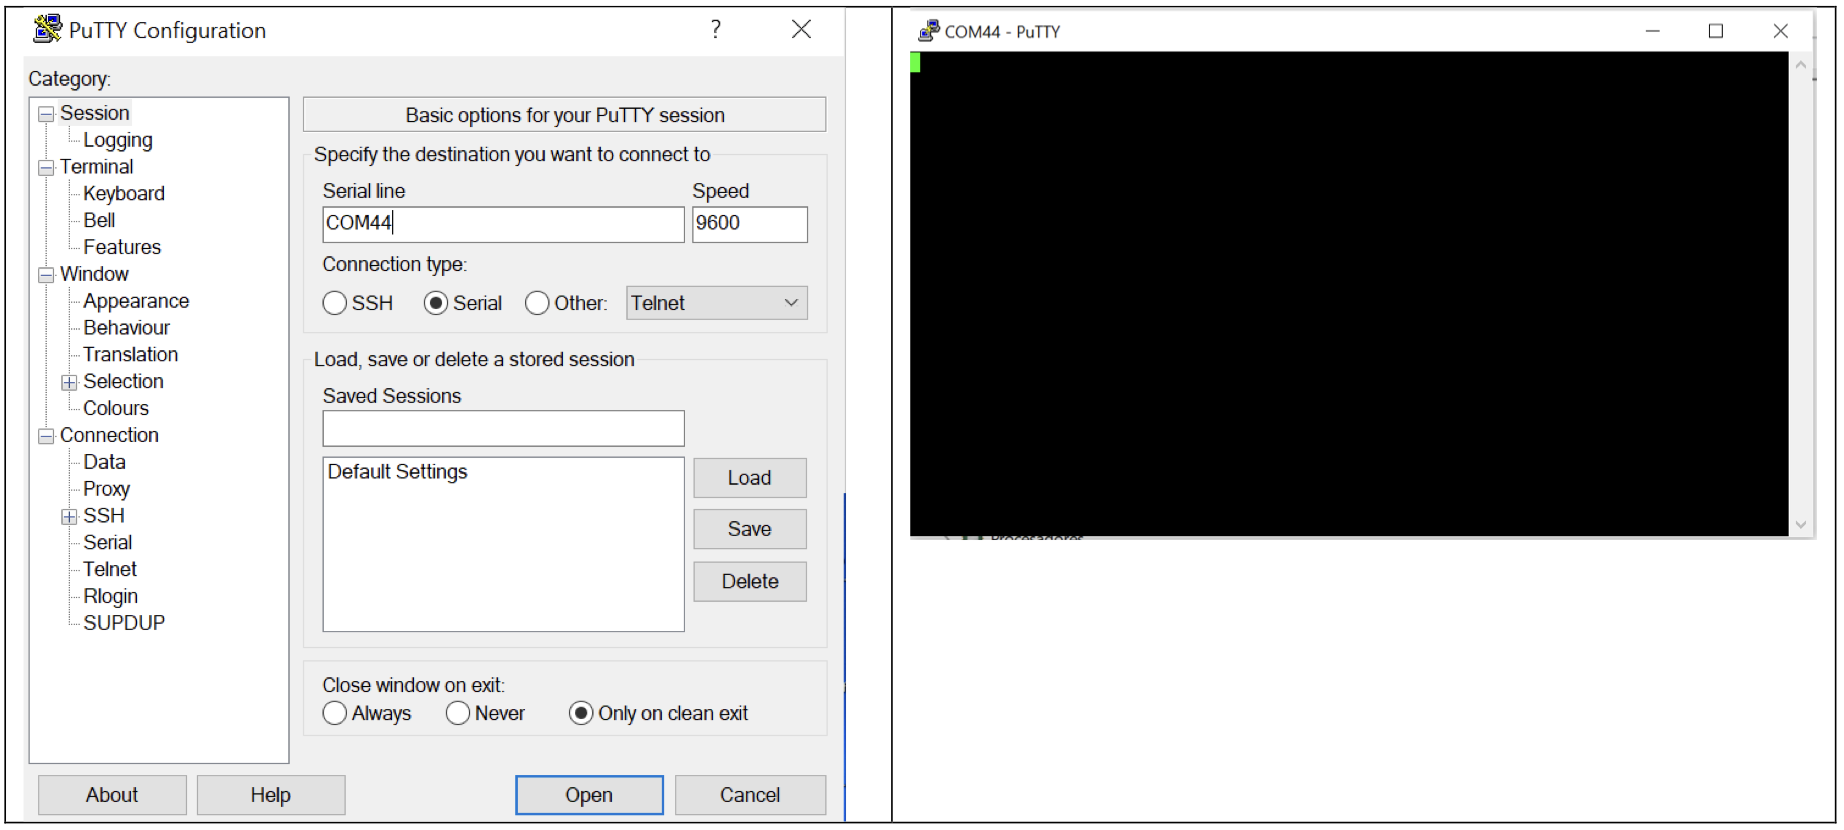
\includegraphics[width=\linewidth]{pics/2-2.png}
        \caption*{Figura 7-5. Configuración de Putty}
    \end{figure}
    \begin{figure}[ht!]
        \centering
        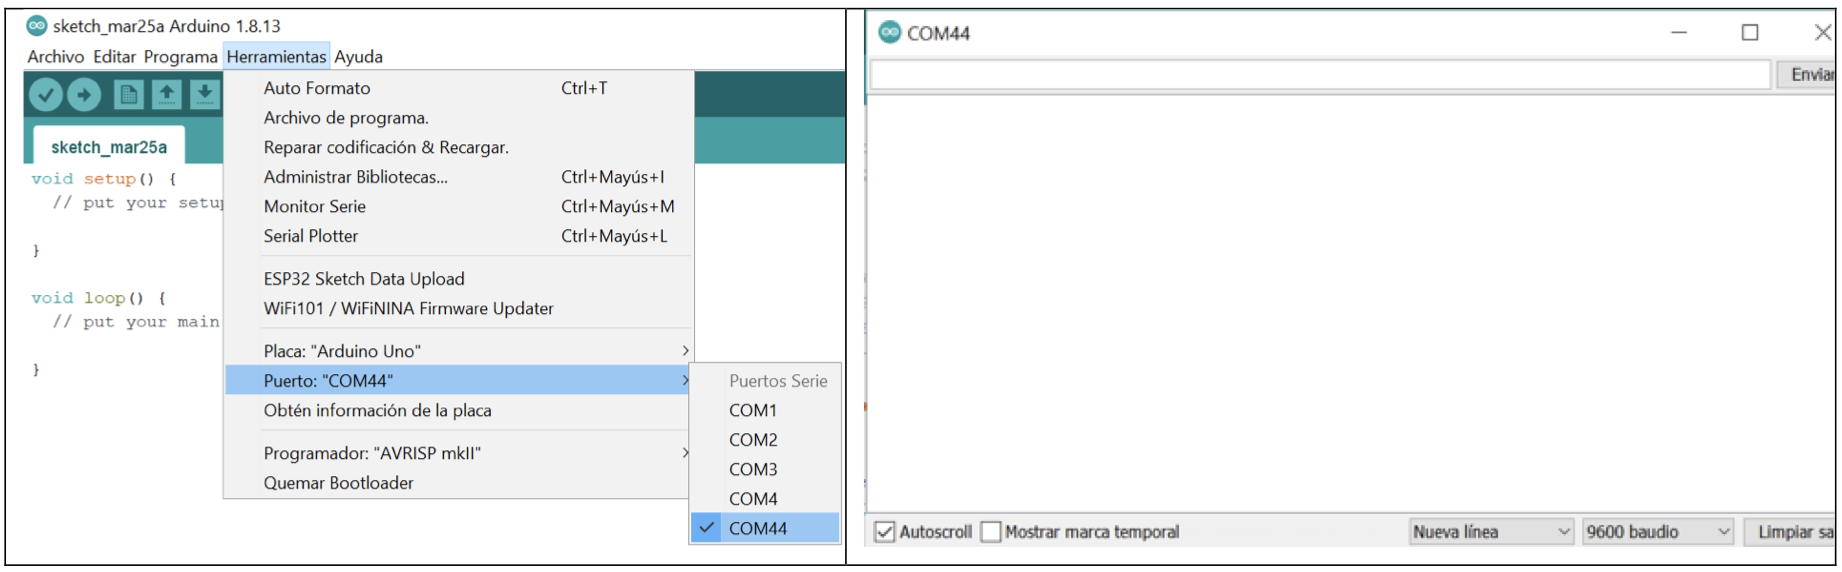
\includegraphics[width=\linewidth]{pics/2-3.png}
        \caption*{Figura 7-6. Configuración en monitor de Arduino}
    \end{figure}

    \item Explicar si existe alguna diferencia en la ejecución y cuál sería el motivo.

\end{enumerate}

\newpage
\subsubsection{Desarrollo}
Sí existe una diferencia en la ejecución al utilizar distintas interfaces como Thonny, PuTTY o el monitor serial de Arduino. La principal diferencia radica en la forma en que cada terminal gestiona la comunicación serial y el envío de caracteres. Algunas terminales envían automáticamente caracteres de fin de línea (como \texttt{\textbackslash n} o \texttt{\textbackslash r\textbackslash n}), mientras que otras requieren configuraciones específicas como baud rate o control de flujo. Esto puede provocar variaciones en la recepción de datos, aunque la lógica del programa permanece correcta.


\begin{figure}[ht!]
    \centering
    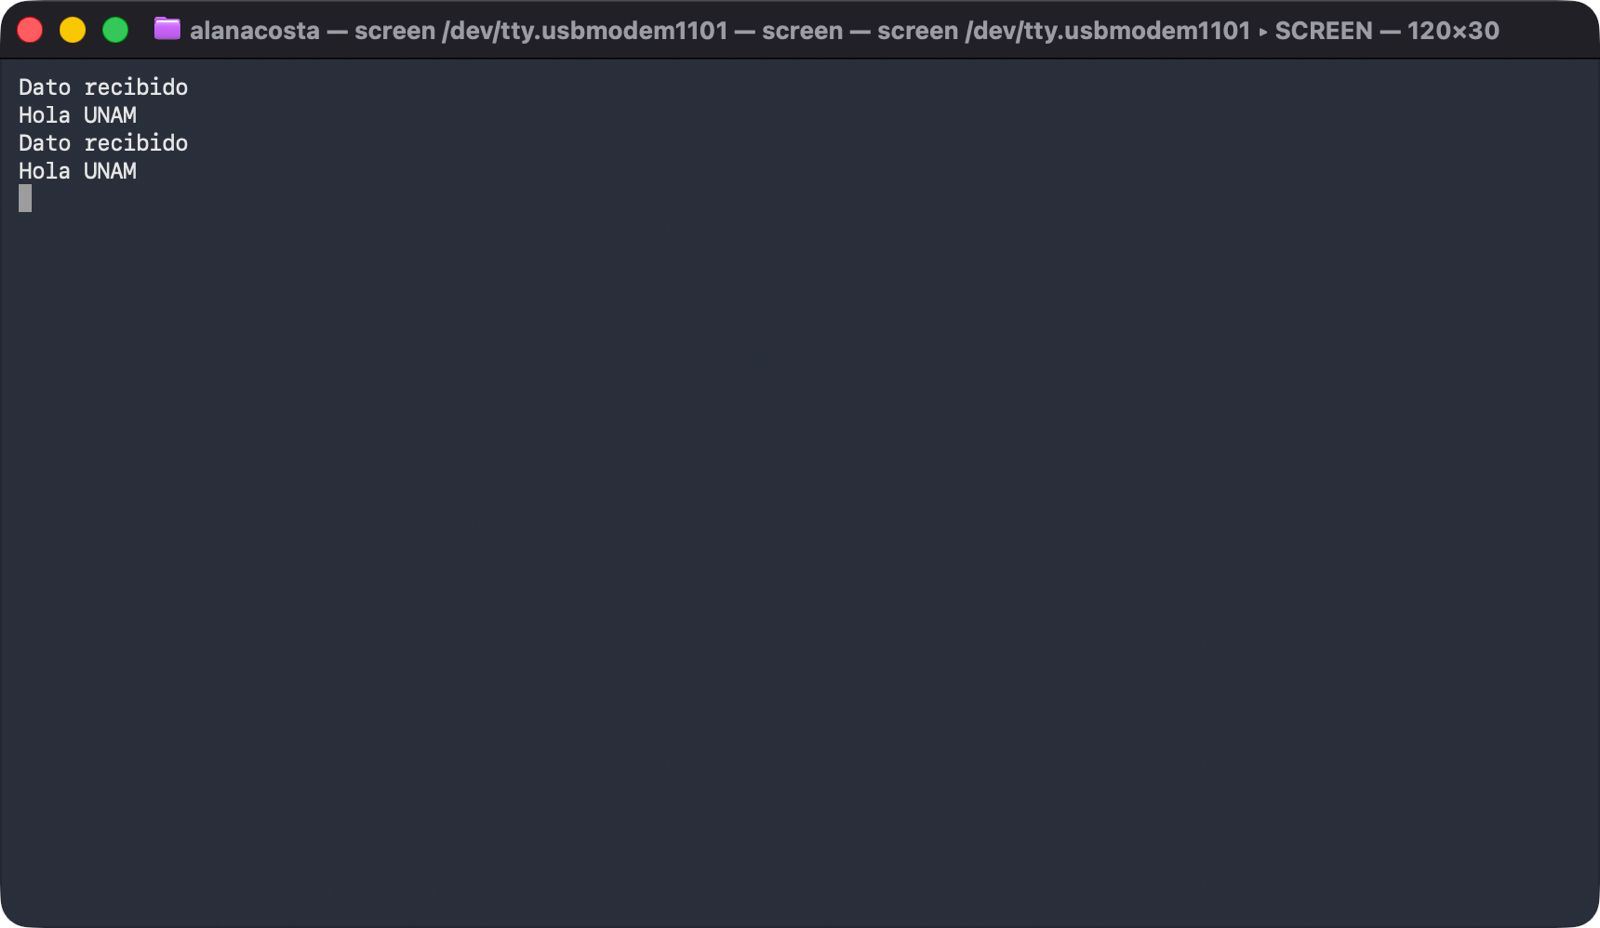
\includegraphics[width=\linewidth]{img/2.png}
    \caption*{Ejecución Ejercicio 2}
\end{figure}

\subsubsection{Análisis de resultados}
Durante la ejecución en diferentes terminales, se observó que el programa mantiene su funcionalidad de recepción y respuesta de datos; sin embargo, la interacción puede variar ligeramente según la herramienta utilizada. En todos los casos, el sistema detectó correctamente la entrada de caracteres y respondió de forma adecuada, confirmando la correcta implementación de la comunicación serial asíncrona. Las diferencias observadas se deben principalmente a la configuración de cada terminal y no afectan el funcionamiento general del programa.


\newpage
%%%%%%%%%%%%%%%%%%%%%%%%%%%%%%%%%%%%%%%%%%%
\subsection{Ejercicio 3}
Utilizando el formato de la actividad 1, realizar un programa que reciba comandos a
través del puerto serie y ejecute las acciones indicadas.
\begin{figure}[ht!]
    \centering
    
\includegraphics[width=1\linewidth]{pics/3.png}
\end{figure}
\subsubsection{Pseudo Código}

\begin{algorithm}[H]
\SetAlgoLined
\caption{Control de LED mediante entrada serial}

Configurar GPIO25 como salida (LED)\;

Inicializar sistema de lectura no bloqueante\;
Registrar entrada estándar\;

Mostrar ``Sistema de control iniciado''\;
Mostrar ``Comandos: 1 para encender, 0 para apagar''\;

Mientras verdadero hacer\;
\Indp
    Verificar si hay datos disponibles en la entrada\;

    \If{hay datos}{
        Leer un carácter\;

        \eIf{carácter = '1'}{
            Encender LED (GPIO25 = 1)\;
            Mostrar ``GPIO25 encendido''\;
        }{
            \If{carácter = '0'}{
                Apagar LED (GPIO25 = 0)\;
                Mostrar ``GPIO25 apagado''\;
            }
        }
    }

    Esperar 0.1 segundos\;
\Indm

\end{algorithm}

\subsubsection{Desarrollo}
\begin{lstlisting}
import select
import sys
import time
import machine

# Configuración del GPIO 25 como salida (Output)
led = machine.Pin(25, machine.Pin.OUT)

# Configuración del objeto poll para monitorear la entrada serial
poll_obj = select.poll()
poll_obj.register(sys.stdin, 1)

sys.stdout.write("Sistema de control iniciado\n")
print("Comandos: '1' para Encender, '0' para Apagar")

while True:
    # Verificamos si hay datos en el búfer de entrada
    if poll_obj.poll(0):
        # Leemos el carácter recibido
        ch = sys.stdin.read(1)
        
        # Lógica de control según el dato recibido
        if ch == '1':
            led.value(1)  # GPIO25 = ON
            sys.stdout.write("Acción: GPIO25 encendido (ON)\n")
        
        elif ch == '0':
            led.value(0)  # GPIO25 = OFF
            sys.stdout.write("Acción: GPIO25 apagado (OFF)\n")
            
        # Nota: Los caracteres como '\n' (Enter) son ignorados 
        # al no coincidir con '1' o '0'.
    
    # Pausa para estabilidad del sistema
    time.sleep(0.1)
\end{lstlisting}

\begin{figure}[ht!]
    \centering
    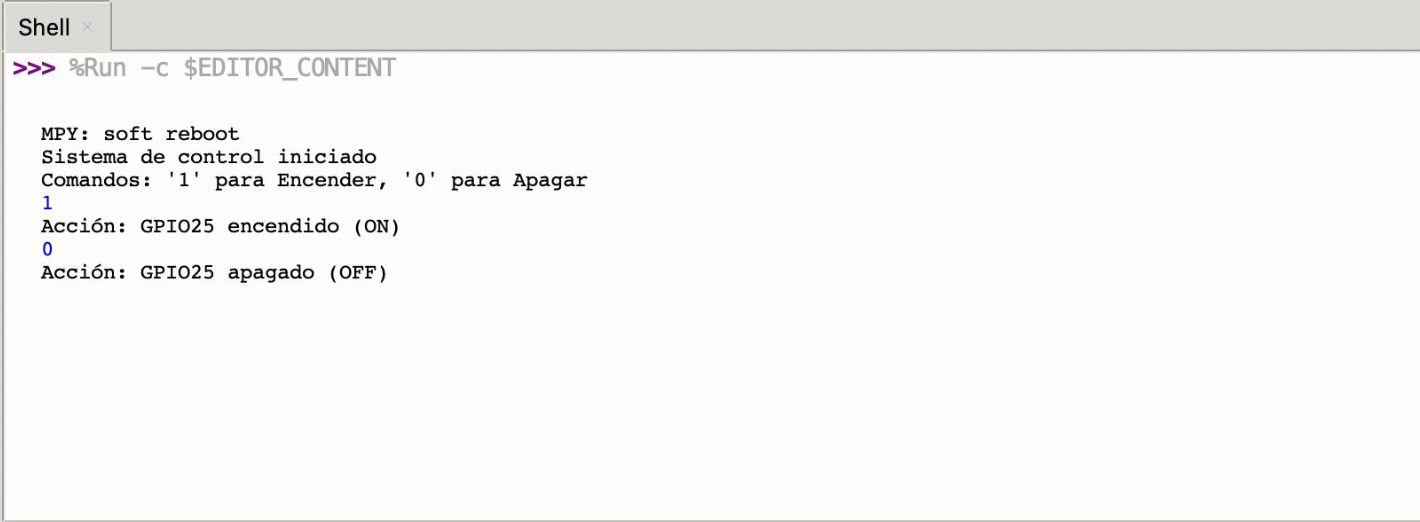
\includegraphics[width=\linewidth]{img/3-1.png}
    \caption*{Ejecución Ejercicio 3}
\end{figure}

\newpage
\begin{figure}[ht!]
    \centering
    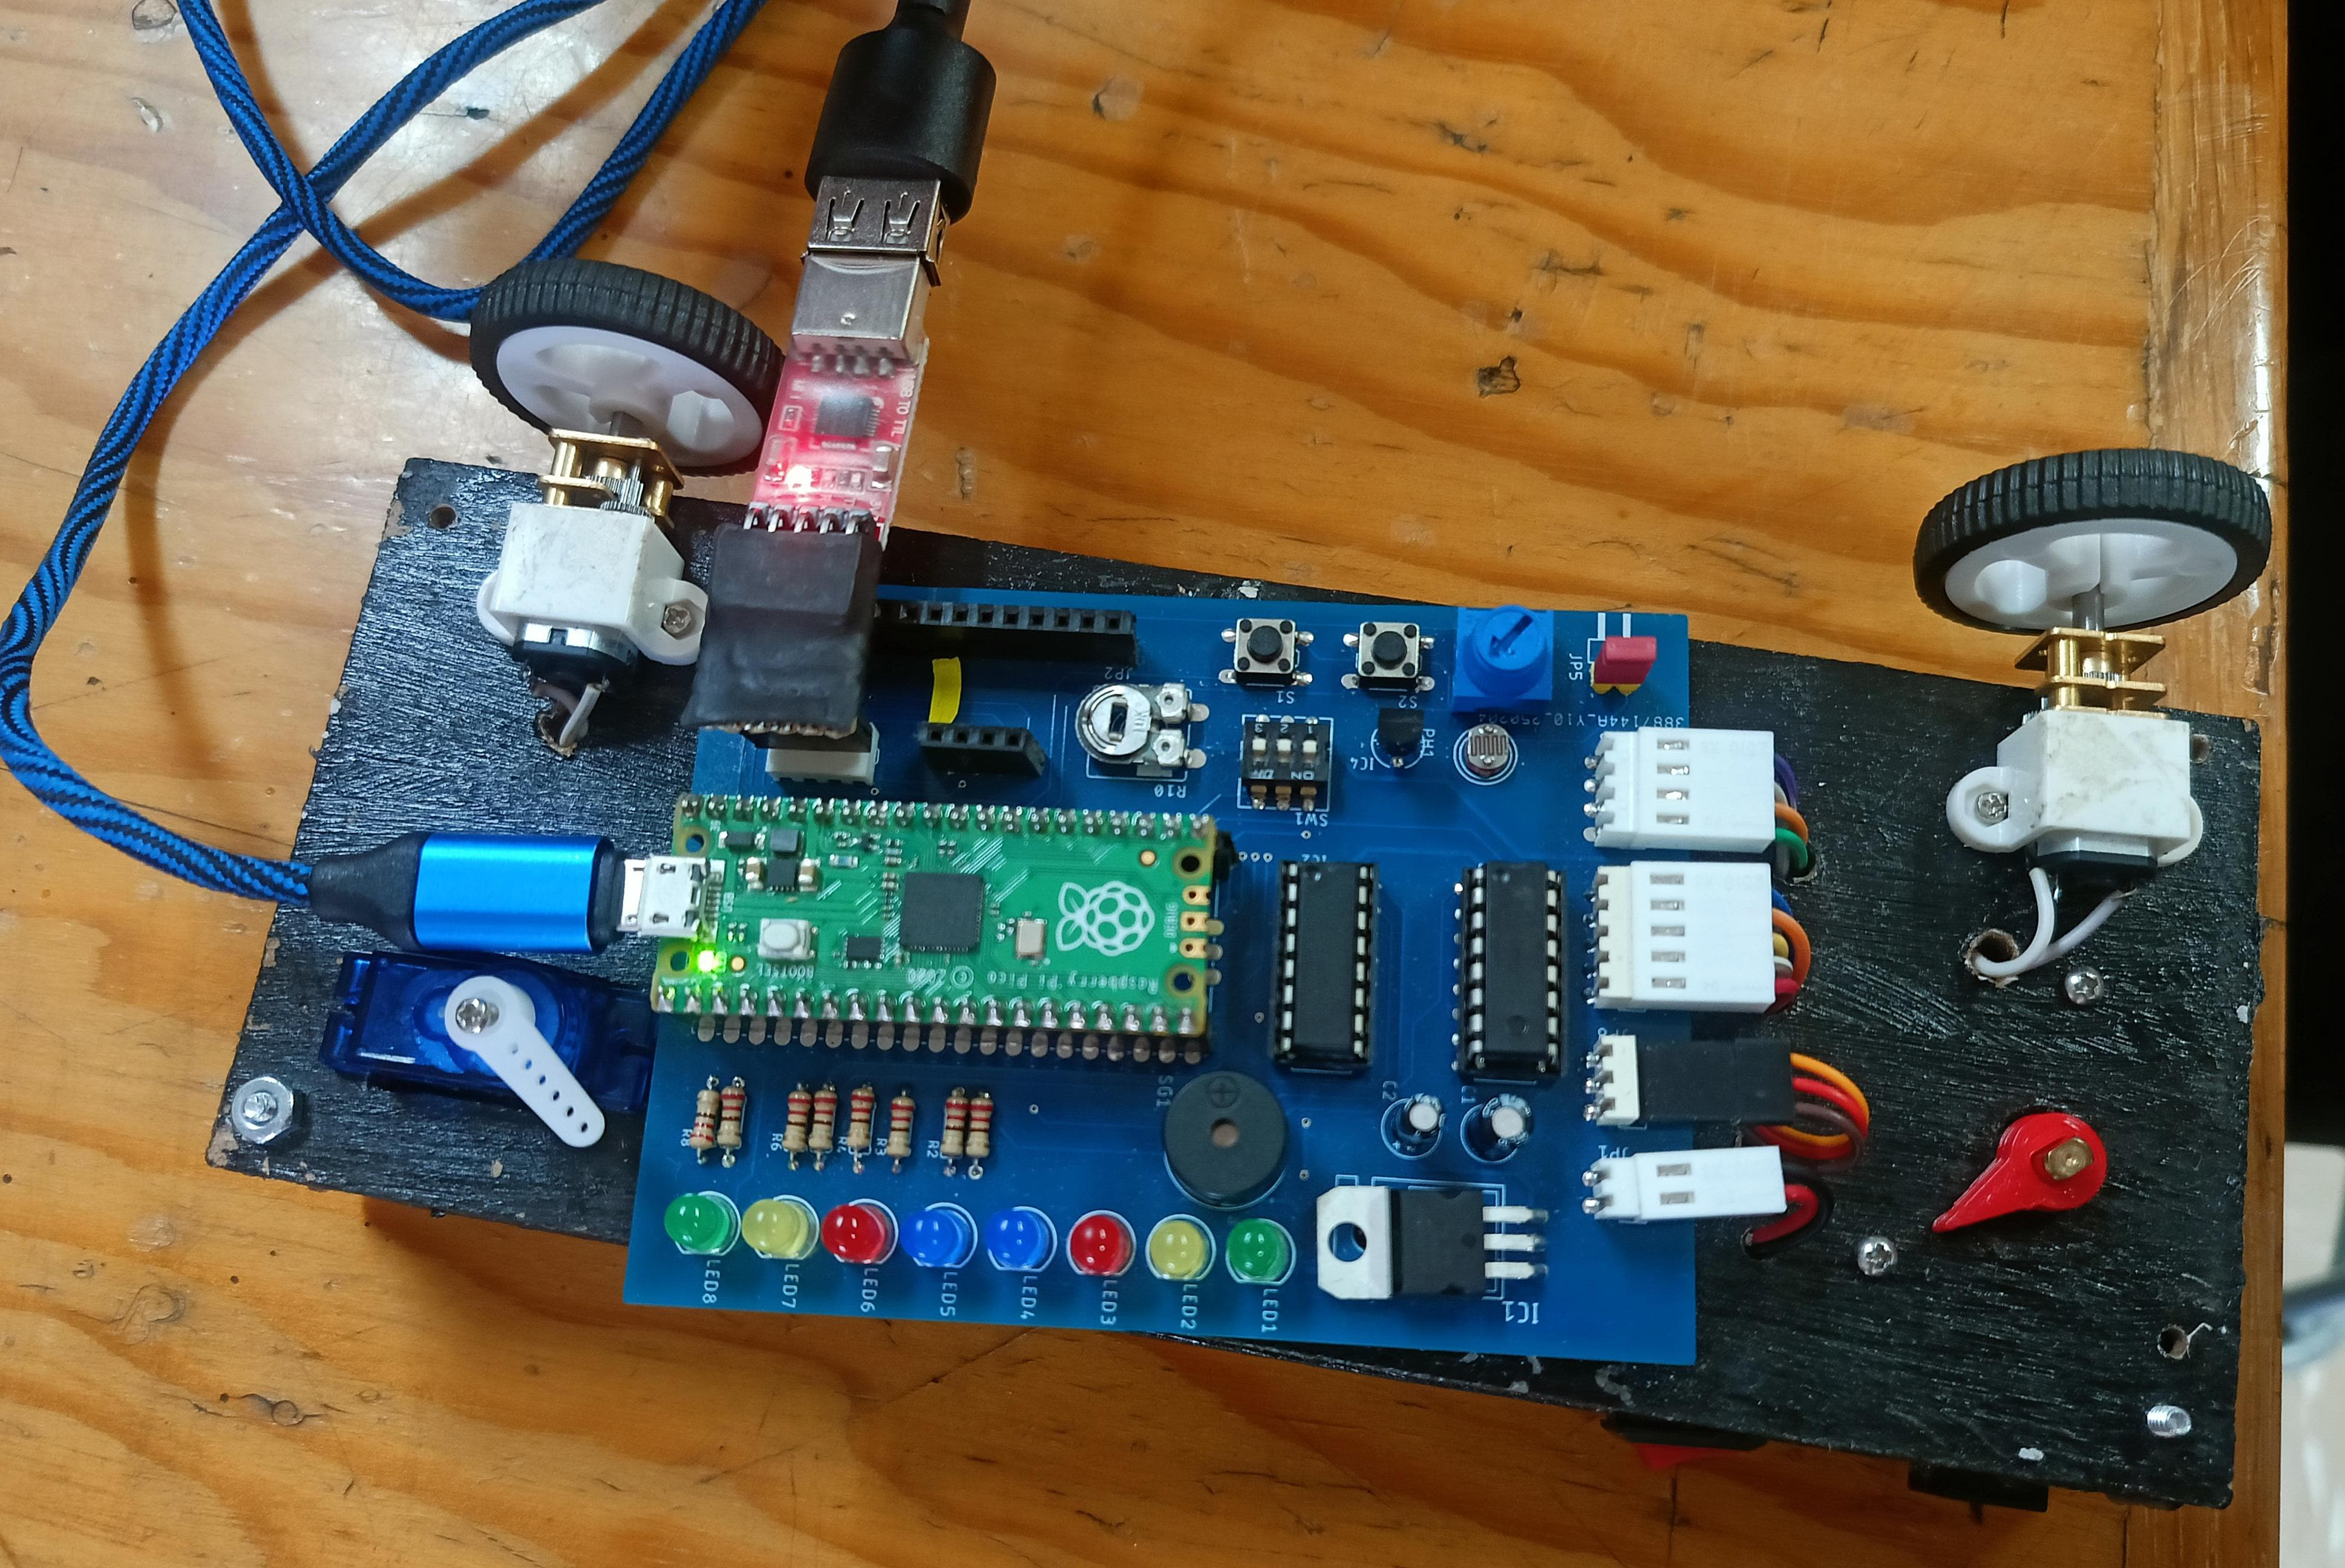
\includegraphics[width=0.8\linewidth]{img/3-2.jpeg}
    \caption*{Raspberry Pi Ejercicio 3}
\end{figure}


\subsubsection{Análisis de resultados}
El sistema respondió correctamente a los comandos enviados desde la terminal, permitiendo controlar el estado del LED mediante caracteres específicos. Se comprobó que la lectura no bloqueante evitó interrupciones en la ejecución del programa, mientras que la lógica condicional filtró adecuadamente los datos válidos, ignorando caracteres como saltos de línea. La interacción fue inmediata y consistente, demostrando un control eficiente de salidas digitales mediante comunicación serial.


\newpage
%%%%%%%%%%%%%%%%%%%%%%%%%%%%%%%%%%%%%%%%%%%
\subsection{Ejercicio 4}
Realizar el siguiente procedimiento:

\begin{itemize}
    \item [a.] Escribir el siguiente programa.
    \item [b.] Comentar el código e indicar que hace.
    \item [c.] Conectar el módulo CP2102.
    \item [d.] Ubicar el puerto asignado.
    \item [e.] Comprobar el funcionamiento
\end{itemize}

\begin{lstlisting}
from machine import Pin, UART
import time

uart = UART(0, baudrate=9600, tx=Pin(16), rx=Pin(17))
uart.init(bits=8, parity=None, stop=1)
led = Pin(25, Pin.OUT)
uart.write('Inicia Comunicacion Serie')
while True:
    if uart.any() > 0:
        data = uart.read()
        uart.write(data)
        led.toggle()
        time.sleep(1)
\end{lstlisting}
\subsubsection{Pseudo Código}

\begin{algorithm}[H]
\SetAlgoLined
\caption{Comunicación UART con control de LED}

Configurar UART en puerto 0 con baudrate 9600\;
Configurar pines TX y RX\;

Configurar LED en GPIO25 como salida\;

Enviar mensaje ``Inicia Comunicación Serie''\;

Mientras verdadero hacer\;
\Indp
    \If{hay datos disponibles en UART}{
        Leer datos recibidos\;
        Enviar de regreso los mismos datos (eco)\;
        Cambiar estado del LED (toggle)\;
        Esperar 1 segundo\;
    }
\Indm

\end{algorithm}


\subsubsection{Desarrollo}
\begin{lstlisting}
from machine import Pin, UART
import time

# Inicializa la UART0 con velocidad de 9600 baudios
# TX en GPIO16 y RX en GPIO17
uart = UART(0, baudrate=9600, tx=Pin(16), rx=Pin(17))

# Configuración adicional de la UART: 8 bits, sin paridad, 1 bit de parada
uart.init(bits=8, parity=None, stop=1)

# Configura el LED en GPIO25 como salida
led = Pin(25, Pin.OUT)

# Envía un mensaje inicial por la UART
uart.write('Inicia Comunicacion Serie')

while True:
    # Verifica si hay datos disponibles en el buffer de recepción
    if uart.any() > 0:
        
        # Lee los datos recibidos
        data = uart.read()
        
        # Envía de regreso los mismos datos (eco)
        uart.write(data)
        
        # Cambia el estado del LED (encendido/apagado)
        led.toggle()
        
        # Espera 1 segundo para evitar cambios muy rápidos
        time.sleep(1)
\end{lstlisting}

\begin{figure}[ht!]
    \centering
    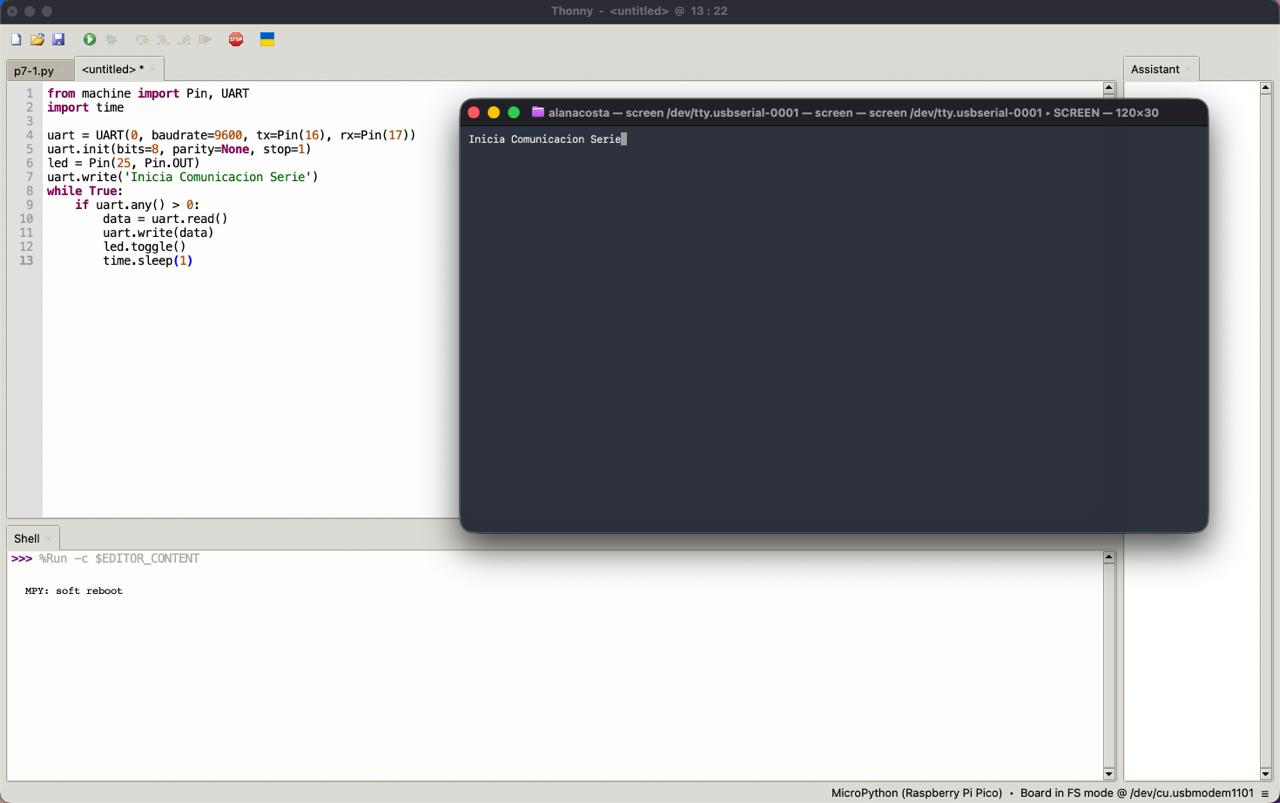
\includegraphics[width=\linewidth]{img/4.png}
    \caption*{Ejecución Ejercicio 4}
\end{figure}


\subsubsection{Análisis de resultados}
Durante la implementación de la comunicación UART con el módulo CP2102, se observó un funcionamiento correcto en la transmisión y recepción de datos. El programa logró realizar un eco de los datos recibidos, confirmando la integridad de la comunicación. Además, el cambio de estado del LED permitió visualizar físicamente la recepción de información. El retardo implementado evitó cambios demasiado rápidos, mejorando la estabilidad del sistema.



\newpage
%%%%%%%%%%%%%%%%%%%%%%%%%%%%%%%%%%%%%%%%%%%
\subsection{Ejercicio 5}
Siguiendo el procedimiento de la actividad No. 4; realizar un programa que ejecute las acciones indicadas.
\begin{figure}[ht!]
    \centering
    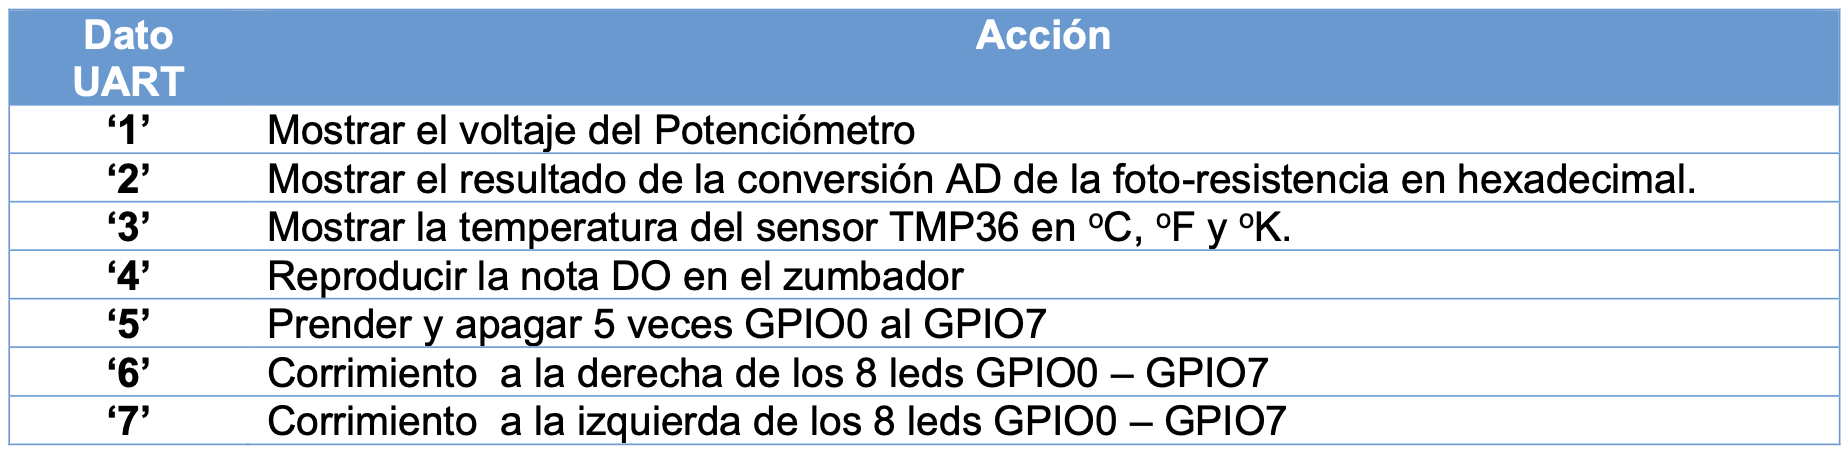
\includegraphics[width=0.7\linewidth]{pics/5.png}
\end{figure}

\subsubsection{Pseudo Código}

\begin{algorithm}[H]
\SetAlgoLined
\caption{Sistema multitarea con UART}

Configurar UART, ADC (pot, LDR, temperatura)\;
Configurar LEDs (GPIO 0–7) y buzzer\;

Mostrar ``Sistema iniciado''\;

Mientras verdadero hacer\;
\Indp
    \If{hay comando en UART}{
        Leer comando\;

        \eIf{cmd = '1'}{
            Leer potenciómetro y enviar voltaje\;
        }{
        \eIf{cmd = '2'}{
            Leer LDR y enviar valor en hexadecimal\;
        }{
        \eIf{cmd = '3'}{
            Leer temperatura y enviar en C, F, K\;
        }{
        \eIf{cmd = '4'}{
            Activar buzzer (nota DO)\;
        }{
        \eIf{cmd = '5'}{
            Parpadear LEDs\;
        }{
        \eIf{cmd = '6'}{
            Corrimiento de LEDs a la derecha\;
        }{
        \If{cmd = '7'}{
            Corrimiento de LEDs a la izquierda\;
        }}}}}}}
    }
\Indm

\end{algorithm}

\subsubsection{Desarrollo}
\begin{lstlisting}
from machine import Pin, UART, ADC, PWM
import time

# 1. Configuración de UART (igual que Actividad 4)
uart = UART(0, baudrate=9600, tx=Pin(16), rx=Pin(17))
uart.init(bits=8, parity=None, stop=1)

# 2. Configuración de Entradas Analógicas (ADC)
pot = ADC(26)      # Potenciómetro
ldr = ADC(27)      # Foto-resistencia
tmp36 = ADC(28)    # Sensor de temperatura

# 3. Configuración de Salidas (LEDs GPIO 0 al 7)
led_pins = [Pin(i, Pin.OUT) for i in range(8)]

# 4. Configuración del Zumbador (PWM)
buzzer = PWM(Pin(15))
buzzer.duty_u16(0) # Iniciamos en silencio

def apagar_leds():
    for led in led_pins:
        led.value(0)

uart.write('Sistema Multitarea Iniciado. Ingrese comando (1-7):\r\n')

while True:
    if uart.any() > 0:
        cmd = uart.read().decode('utf-8').strip()
        
        # --- ACCIÓN 1: Voltaje del Potenciómetro ---
        if cmd == '1':
            reading = pot.read_u16()
            voltage = reading * (3.3 / 65535)
            uart.write('Voltaje Pot: {:.2f}V\r\n'.format(voltage))

        # --- ACCIÓN 2: LDR en Hexadecimal ---
        elif cmd == '2':
            val_ldr = ldr.read_u16()
            uart.write('LDR (Hex): {}\r\n'.format(hex(val_ldr)))

        # --- ACCIÓN 3: Temperatura TMP36 ---
        elif cmd == '3':
            # Conversión de lectura a grados Celsius
            m_voltios = tmp36.read_u16() * (3300 / 65535)
            celsius = (m_voltios - 500) / 10
            fahrenheit = (celsius * 9/5) + 32
            kelvin = celsius + 273.15
            
            msg = 'Temp: {:.2f}C, {:.2f}F, {:.2f}K\r\n'.format(celsius, fahrenheit, kelvin)
            uart.write(msg)

        # --- ACCIÓN 4: Nota DO en Zumbador ---
        elif cmd == '4':
            uart.write('Reproduciendo DO (261Hz)...\r\n')
            buzzer.freq(261)   # Frecuencia de la nota DO (C4)
            buzzer.duty_u16(32768) # 50% de ciclo de trabajo
            time.sleep(0.5)
            buzzer.duty_u16(0)

        # --- ACCIÓN 5: Parpadeo GPIO 0-7 (5 veces) ---
        elif cmd == '5':
            uart.write('Parpadeando LEDs x5...\r\n')
            for _ in range(5):
                for led in led_pins: led.value(1)
                time.sleep(0.2)
                for led in led_pins: led.value(0)
                time.sleep(0.2)

        # --- ACCIÓN 6: Corrimiento a la derecha ---
        elif cmd == '6':
            uart.write('Corrimiento Derecha (0 -> 7)...\r\n')
            apagar_leds()
            for led in led_pins:
                led.value(1)
                time.sleep(0.1)
                led.value(0)

        # --- ACCIÓN 7: Corrimiento a la izquierda ---
        elif cmd == '7':
            uart.write('Corrimiento Izquierda (7 -> 0)...\r\n')
            apagar_leds()
            for led in reversed(led_pins):
                led.value(1)
                time.sleep(0.1)
                led.value(0)

    time.sleep(0.1)
\end{lstlisting}

\newpage
\begin{figure}[ht!]
    \centering
    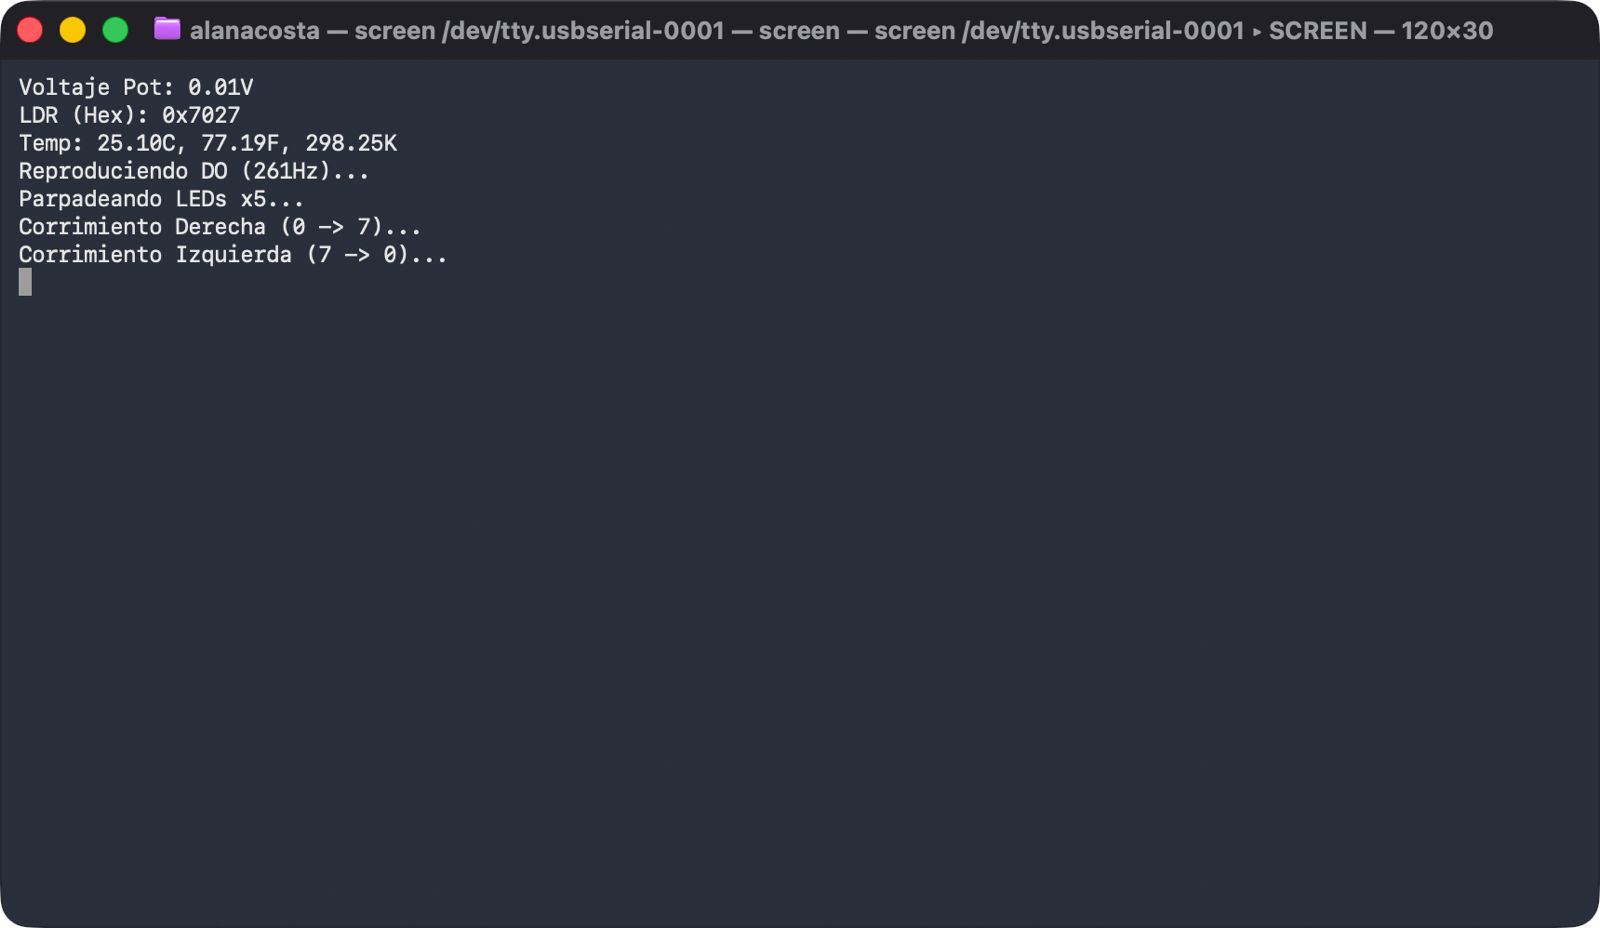
\includegraphics[width=\linewidth]{img/5-1.png}
    \caption*{Ejecución Ejercicio 5}
\end{figure}

\begin{figure}[ht!]
    \centering
    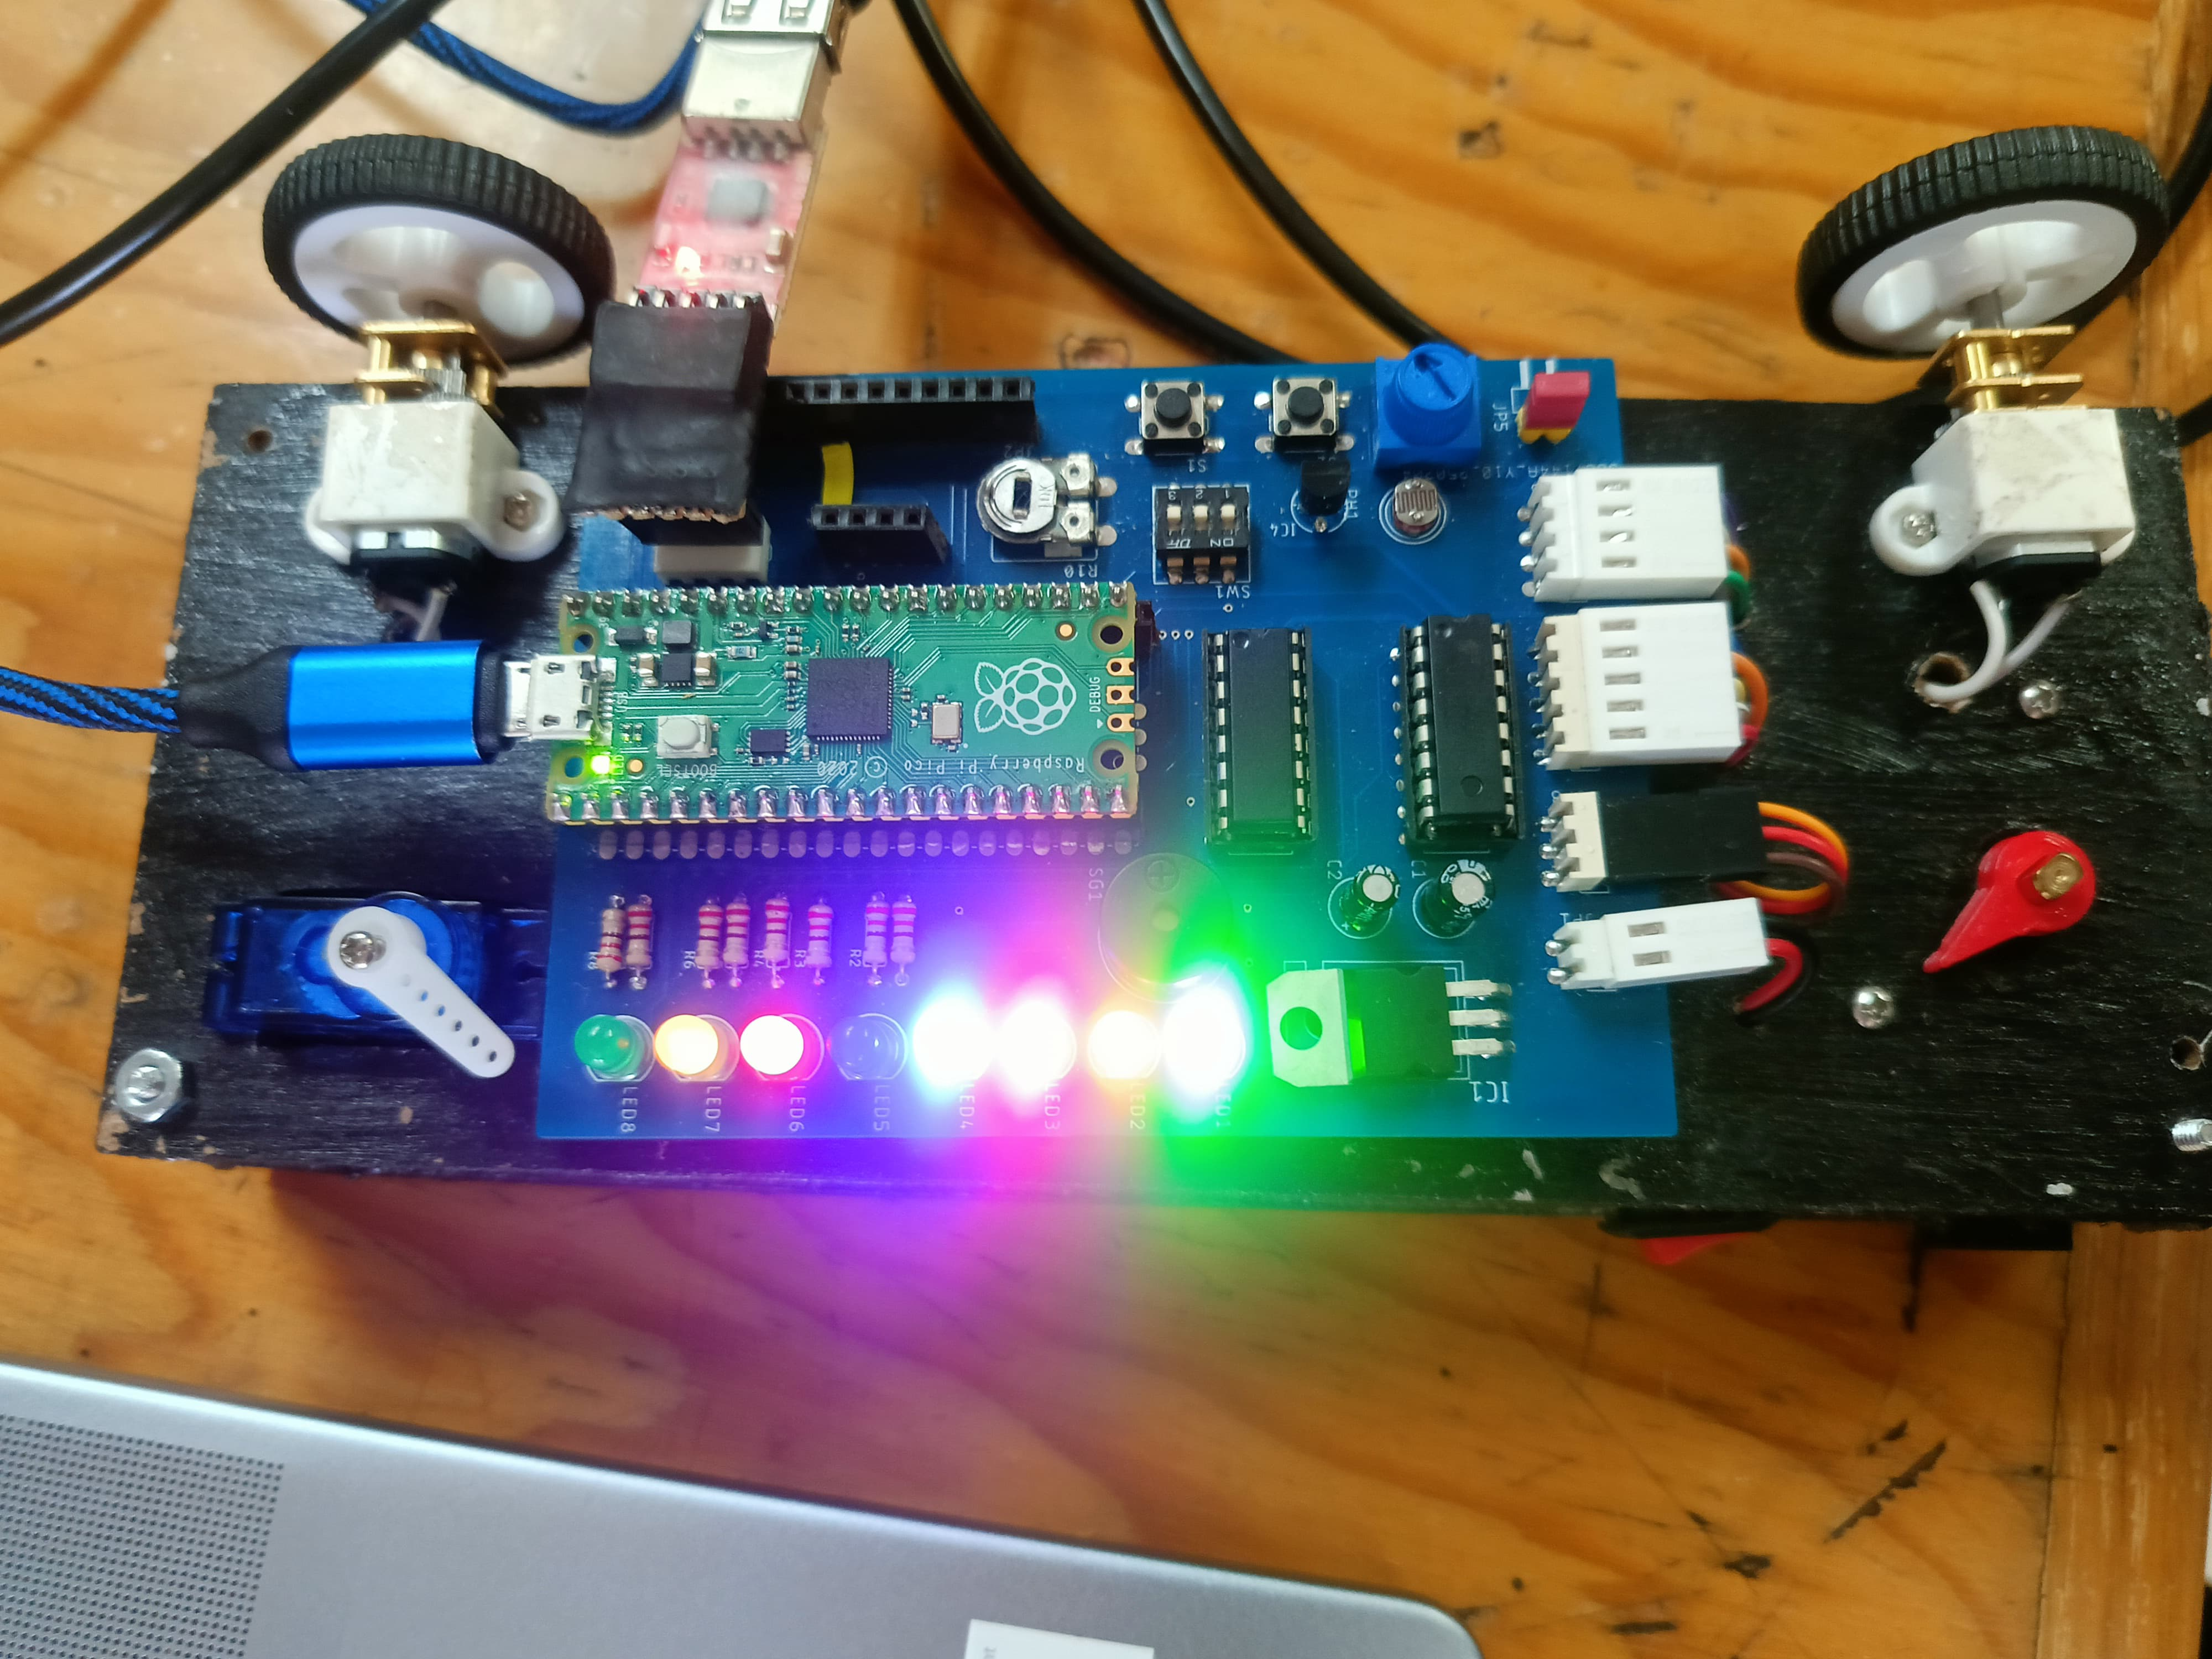
\includegraphics[width=0.8\linewidth]{img/5-2.jpeg}
    \caption*{Raspberry Pi Ejercicio 5}
\end{figure}

\newpage
\subsubsection{Análisis de resultados}
El sistema multitarea mostró un comportamiento adecuado al ejecutar distintas acciones dependiendo del comando recibido. Se verificó la correcta lectura de sensores analógicos (potenciómetro, LDR y temperatura), así como la conversión de datos a diferentes unidades. Las salidas digitales (LEDs) y el buzzer respondieron correctamente, evidenciando la integración de múltiples periféricos en un solo programa. La estructura condicional permitió una ejecución clara y organizada de cada función.



\newpage
%%%%%%%%%%%%%%%%%%%%%%%%%%%%%%%%%%%%%%%%%%%

\subsection{Ejercicio 6}
Conectando el módulo bluetooth, realizar un programa que ejecute las acciones indicadas
en la tabla 7-4.
\begin{figure}[ht!]
    \centering
    
\includegraphics[width=1\linewidth]{pics/6.png}
\end{figure}

\subsubsection{Pseudo Código}

\begin{algorithm}[H]
\SetAlgoLined
\caption{Control de motores por UART (Bluetooth)}

Configurar UART (9600 baudios)\;
Configurar pines de motores (Puente H)\;

Definir función detener motores\;
Definir función para controlar dirección de motores\;

Mostrar ``Sistema listo''\;

Mientras verdadero hacer\;
\Indp
    \If{hay datos en UART}{
        Leer comando y convertir a mayúsculas\;

        \eIf{cmd = 'S'}{
            Detener ambos motores\;
        }{
        \eIf{cmd = 'A'}{
            Ambos motores en sentido horario\;
        }{
        \eIf{cmd = 'T'}{
            Ambos motores en sentido antihorario\;
        }{
        \eIf{cmd = 'D'}{
            Motor 1 horario, Motor 2 antihorario\;
        }{
        \If{cmd = 'I'}{
            Motor 1 antihorario, Motor 2 horario\;
        }}}}}
    }

    Esperar 0.1 segundos\;
\Indm

\end{algorithm}

\newpage
\subsubsection{Desarrollo}
\begin{lstlisting}
from machine import Pin, UART
import time

# 1. Configuración de UART (Bluetooth en GP16 y GP17)
uart = UART(0, baudrate=9600, tx=Pin(16), rx=Pin(17))

# 2. Configuración de Pines para Motores (Puente H)
# Motor 1
m1_a = Pin(2, Pin.OUT)
m1_b = Pin(3, Pin.OUT)
# Motor 2
m2_a = Pin(4, Pin.OUT)
m2_b = Pin(5, Pin.OUT)

# Función para detener ambos motores
def stop():
    m1_a.value(0); m1_b.value(0)
    m2_a.value(0); m2_b.value(0)

# Función para establecer giro (1=Horario, -1=Anti-horario, 0=Paro)
def set_motors(m1_dir, m2_dir):
    # Lógica Motor 1
    if m1_dir == 1:    # Horario
        m1_a.value(1); m1_b.value(0)
    elif m1_dir == -1: # Anti-horario
        m1_a.value(0); m1_b.value(1)
    else:              # Paro
        m1_a.value(0); m1_b.value(0)
        
    # Lógica Motor 2
    if m2_dir == 1:    # Horario
        m2_a.value(1); m2_b.value(0)
    elif m2_dir == -1: # Anti-horario
        m2_a.value(0); m2_b.value(1)
    else:              # Paro
        m2_a.value(0); m2_b.value(0)

uart.write("Control de Motores Listo (A, T, D, I, S)\r\n")

while True:
    if uart.any() > 0:
        # Leemos el comando y lo pasamos a mayúsculas
        comando = uart.read().decode('utf-8').strip().upper()
        
        if comando == 'S':
            stop()
            uart.write("ACCION: PARO - PARO\r\n")
            
        elif comando == 'A':
            set_motors(1, 1)
            uart.write("ACCION: HORARIO - HORARIO\r\n")
            
        elif comando == 'T':
            set_motors(-1, -1)
            uart.write("ACCION: ANTI-HORARIO - ANTI-HORARIO\r\n")
            
        elif comando == 'D':
            set_motors(1, -1)
            uart.write("ACCION: HORARIO - ANTI-HORARIO\r\n")
            
        elif comando == 'I':
            set_motors(-1, 1)
            uart.write("ACCION: ANTI-HORARIO - HORARIO\r\n")

    time.sleep(0.1)
\end{lstlisting}

\begin{figure}[ht!]
    \centering
    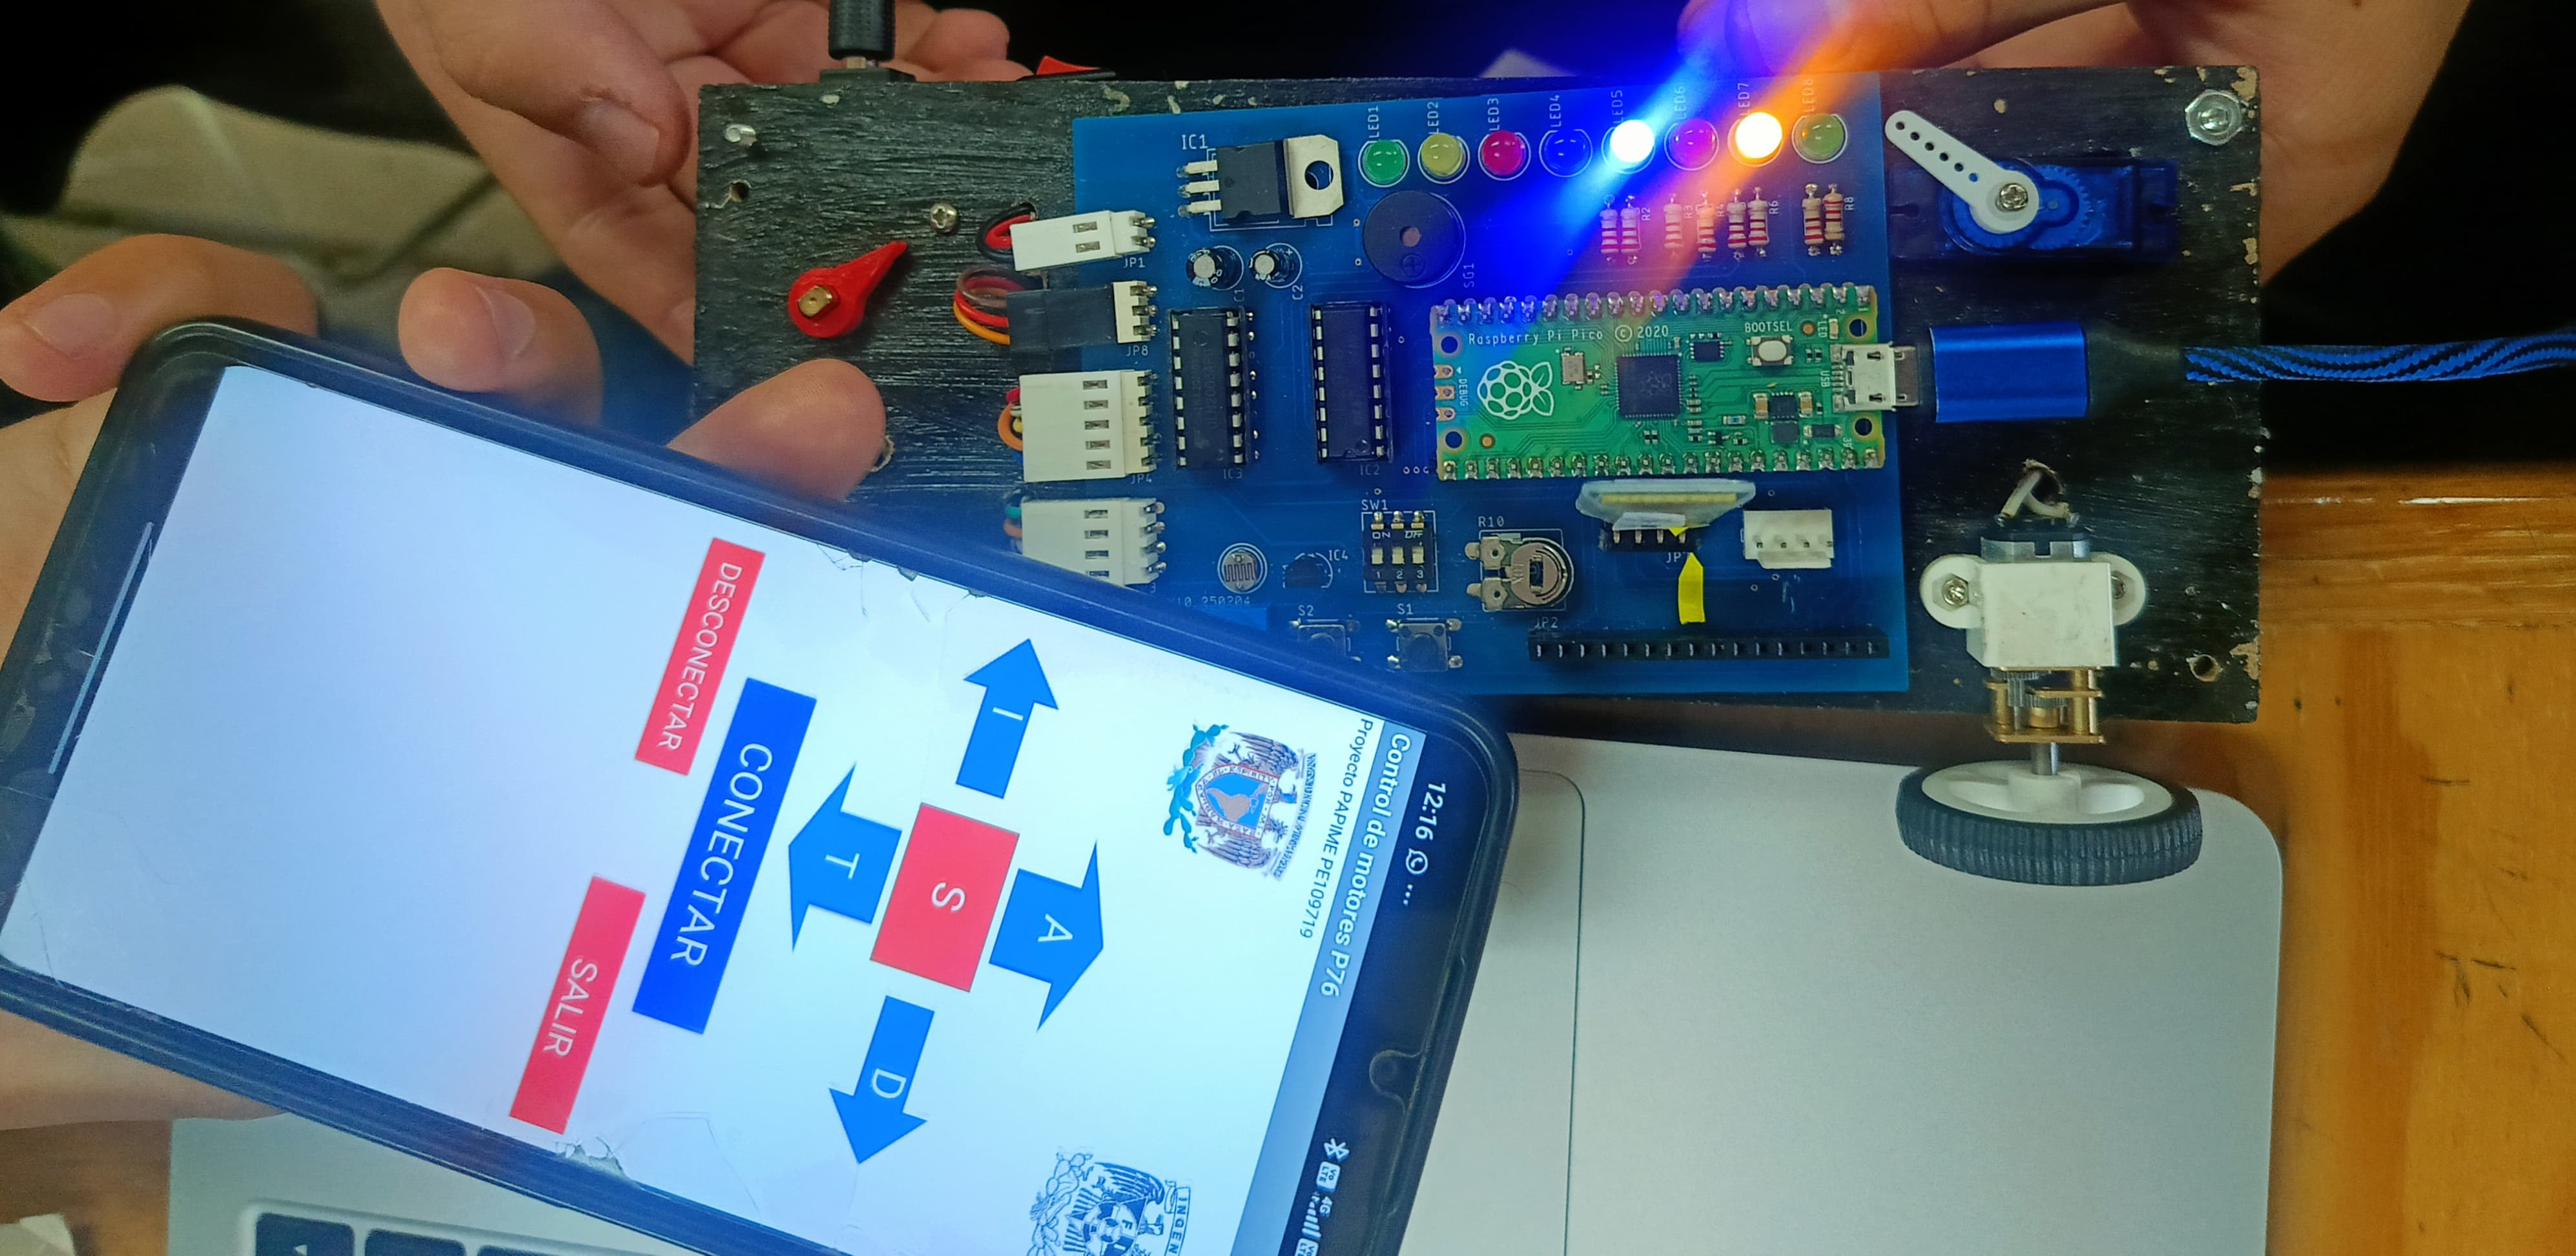
\includegraphics[width=\linewidth]{img/6.jpeg}
    \caption*{Raspberry Pi Ejercicio 6}
\end{figure}

\subsubsection{Análisis de resultados}
El control de motores mediante comunicación Bluetooth fue exitoso, permitiendo ejecutar diferentes movimientos según los comandos enviados. Se comprobó que la lógica implementada en el puente H permitió invertir el sentido de giro de los motores correctamente. La respuesta del sistema fue inmediata, lo que demuestra una comunicación eficiente. Asimismo, la normalización de los comandos (uso de mayúsculas) evitó errores de interpretación.



\newpage
%%%%%%%%%%%%%%%%%%%%%%%%%%%%%%%%%%%%%%%%%%%
\subsection{Ejercicio 7}
Realizar un programa que controle el funcionamiento de los motores de Corriente Directa de la practica 5, por medio de la comunicación serie empleando el módulo Bluetooth.

\begin{figure}[ht!]
    \centering
    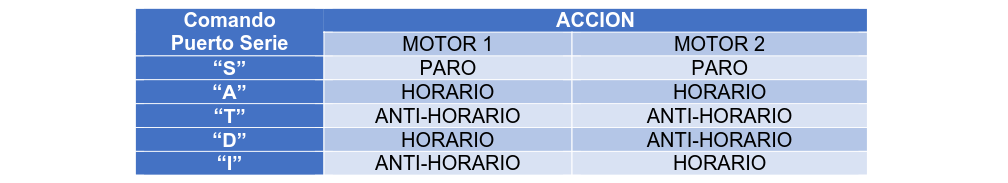
\includegraphics[width=1\linewidth]{pics/7.png}
\end{figure}

\subsubsection{Pseudo Código}

\begin{algorithm}[H]
\SetAlgoLined
\caption{Control de motores con PWM por UART}

Configurar UART (Bluetooth)\;
Configurar pines de dirección de ambos motores\;
Configurar PWM para control de velocidad\;

Definir velocidad máxima\;
Definir función para controlar motores (dirección y velocidad)\;

Mostrar ``Sistema listo''\;

Mientras verdadero hacer\;
\Indp
    \If{hay datos en UART}{
        Leer comando y convertir a mayúsculas\;

        \eIf{cmd = 'S'}{
            Detener ambos motores\;
        }{
        \eIf{cmd = 'A'}{
            Ambos motores avanzan (máxima velocidad)\;
        }{
        \eIf{cmd = 'T'}{
            Ambos motores retroceden\;
        }{
        \eIf{cmd = 'D'}{
            Giro a la derecha\;
        }{
        \If{cmd = 'I'}{
            Giro a la izquierda\;
        }}}}}
    }

    Esperar 0.1 segundos\;
\Indm

\end{algorithm}

\newpage
\subsubsection{Desarrollo}
\begin{lstlisting}
from machine import Pin, UART, PWM
import time

# 1. Configuración de UART (Bluetooth en GP16 y GP17)
uart = UART(0, baudrate=9600, tx=Pin(16), rx=Pin(17))

# 2. Configuración Motor 1 (Según imagen)
m1_dir1 = Pin(0, Pin.OUT)  # DIR1_M1
m1_dir2 = Pin(1, Pin.OUT)  # DIR2_M1
m1_en = PWM(Pin(20))       # EN_M1 (Habilitación/Velocidad)
m1_en.freq(1000)           # Frecuencia de 1kHz para el motor

# 3. Configuración Motor 2 (Según imagen)
m2_dir1 = Pin(2, Pin.OUT)  # DIR1_M2
m2_dir2 = Pin(3, Pin.OUT)  # DIR2_M2
m2_en = PWM(Pin(19))       # EN_M2 (Habilitación/Velocidad)
m2_en.freq(1000)

def set_motors(d1, d2, d3, d4, speed_m1, speed_m2):
    # Motor 1
    m1_dir1.value(d1)
    m1_dir2.value(d2)
    m1_en.duty_u16(speed_m1)
    # Motor 2
    m2_dir1.value(d3)
    m2_dir2.value(d4)
    m2_en.duty_u16(speed_m2)

# Velocidad máxima (ciclo de trabajo al 100%)
MAX_SPEED = 65535 

uart.write("Control de Motores UNAM - Listo\r\n")

while True:
    if uart.any() > 0:
        comando = uart.read().decode('utf-8').strip().upper()
        
        if comando == 'S':  # PARO - PARO
            set_motors(0, 0, 0, 0, 0, 0)
            uart.write("ACCION: PARO\r\n")
            
        elif comando == 'A':  # HORARIO - HORARIO
            set_motors(1, 0, 1, 0, MAX_SPEED, MAX_SPEED)
            uart.write("ACCION: AVANZAR (H-H)\r\n")
            
        elif comando == 'T':  # ANTI-HORARIO - ANTI-HORARIO
            set_motors(0, 1, 0, 1, MAX_SPEED, MAX_SPEED)
            uart.write("ACCION: RETROCEDER (AH-AH)\r\n")
            
        elif comando == 'D':  # HORARIO - ANTI-HORARIO
            set_motors(1, 0, 0, 1, MAX_SPEED, MAX_SPEED)
            uart.write("ACCION: DERECHA (H-AH)\r\n")
            
        elif comando == 'I':  # ANTI-HORARIO - HORARIO
            set_motors(0, 1, 1, 0, MAX_SPEED, MAX_SPEED)
            uart.write("ACCION: IZQUIERDA (AH-H)\r\n")

    time.sleep(0.1)
\end{lstlisting}

\begin{figure}[ht!]
    \centering
    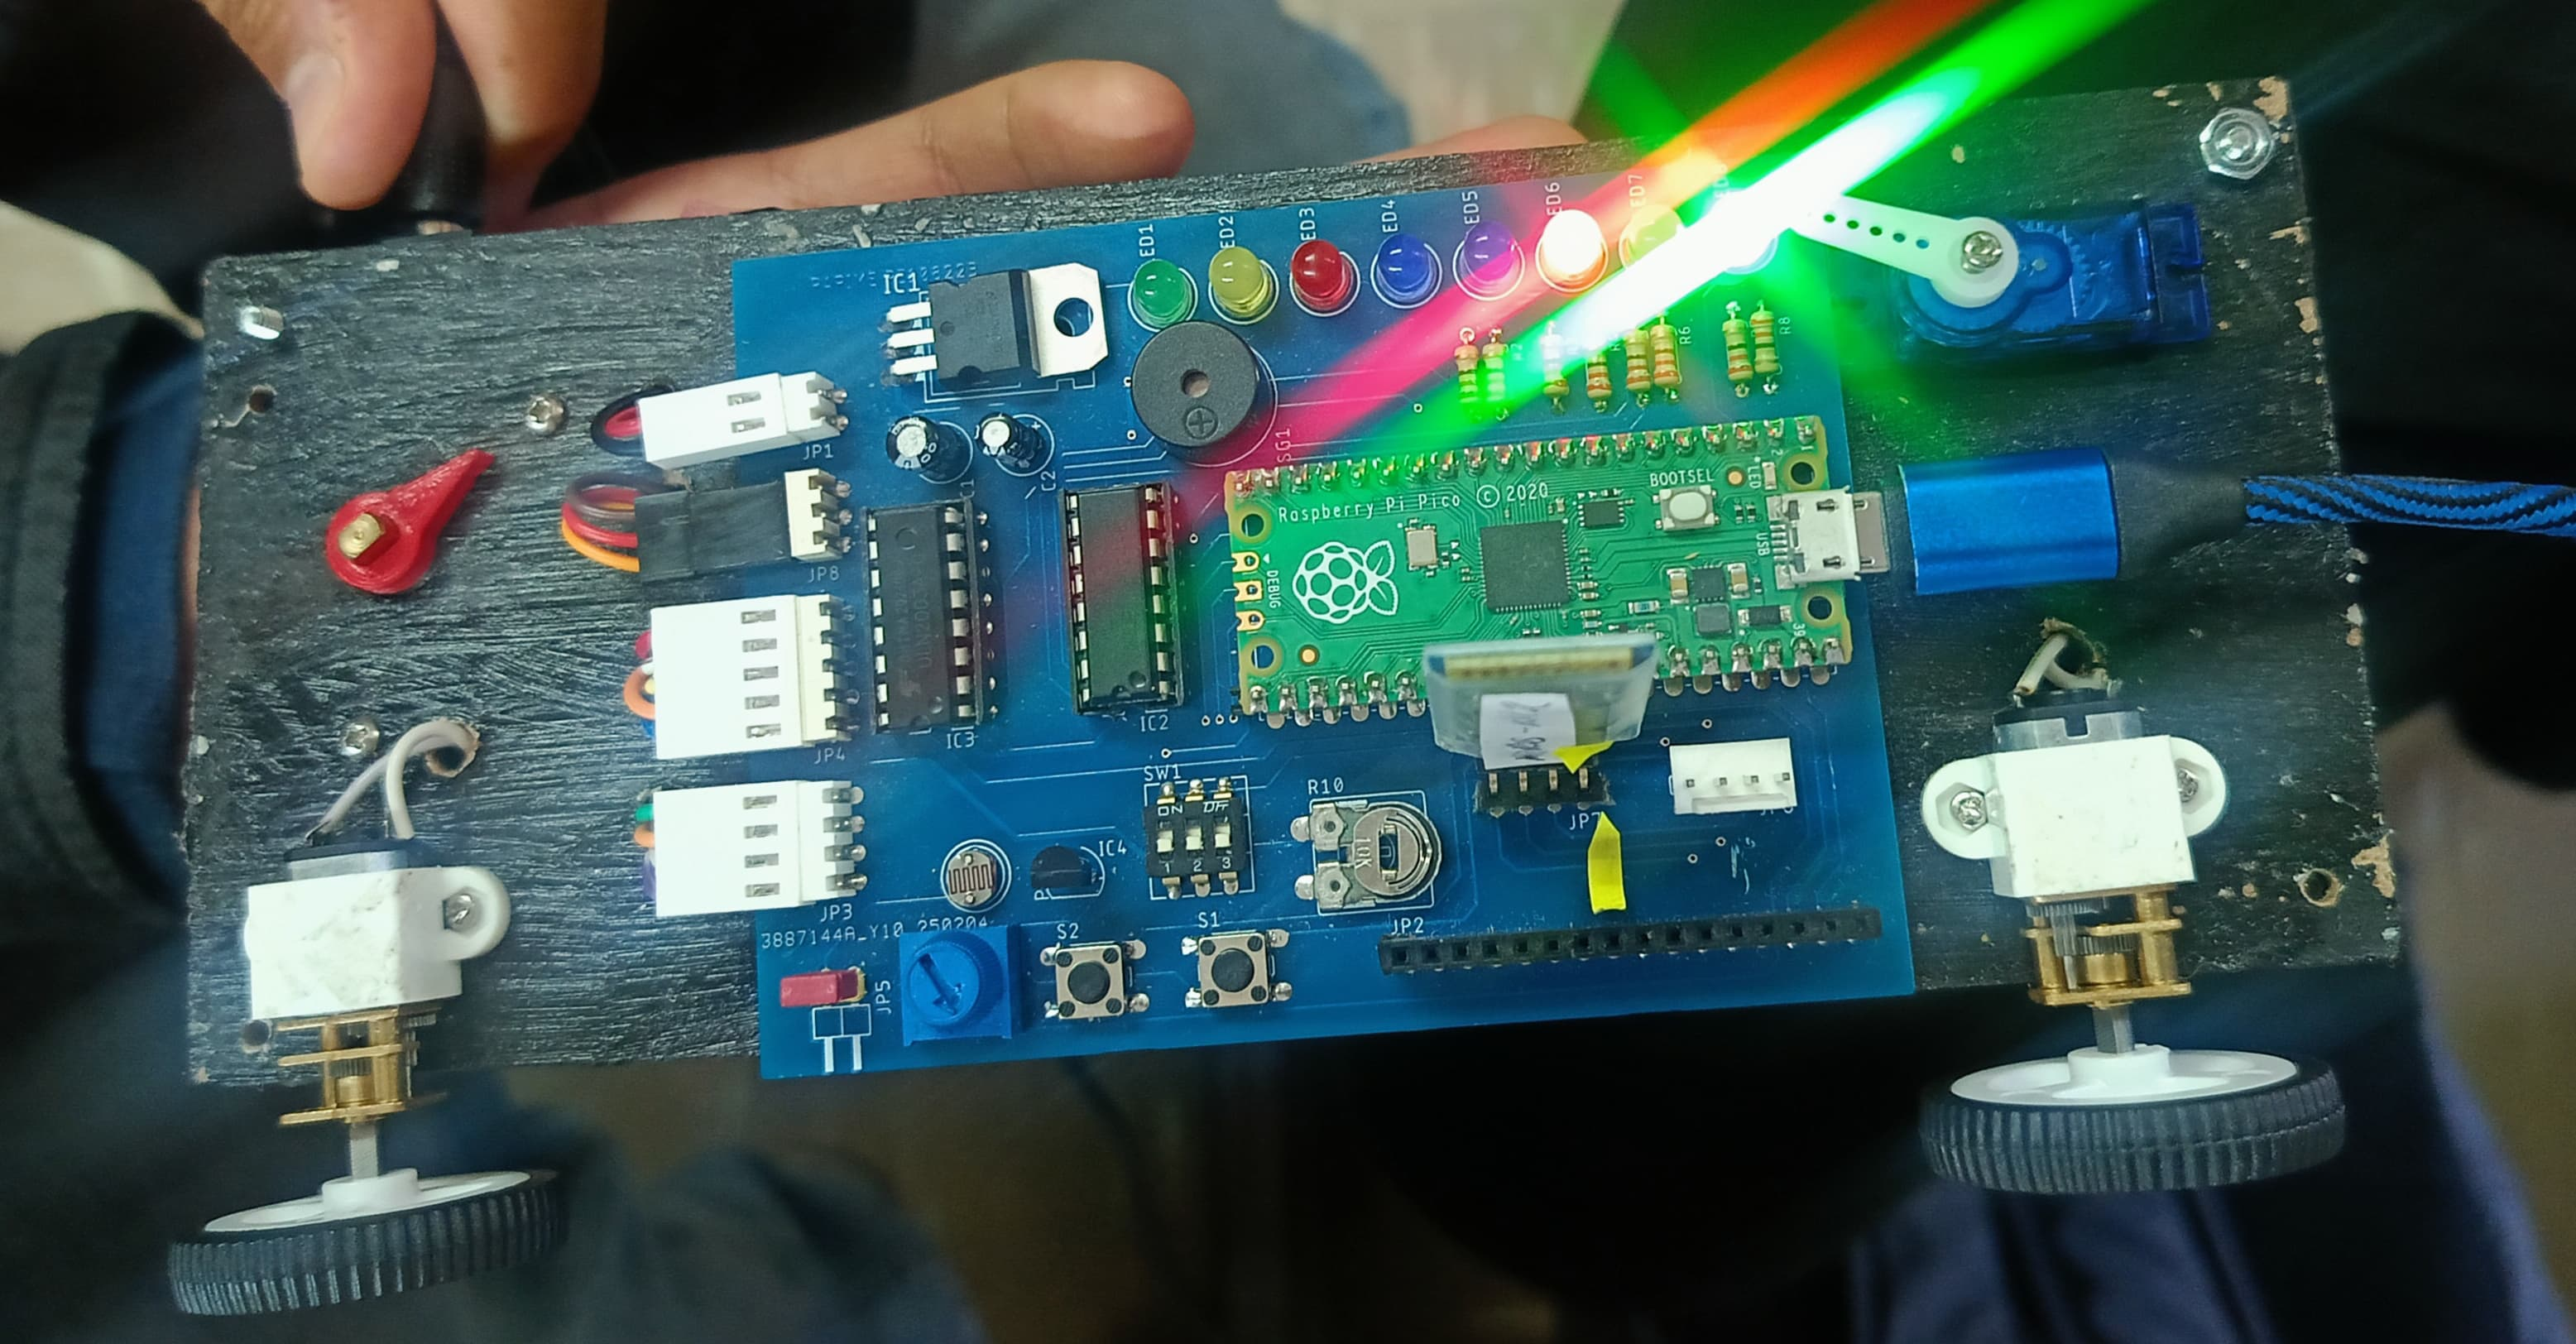
\includegraphics[width=\linewidth]{img/7.jpeg}
    \caption*{Raspberry Pi Ejercicio 7}
\end{figure}

\subsubsection{Análisis de resultados}
La incorporación de PWM permitió un control más avanzado de los motores, no solo en dirección sino también en velocidad. Se observó que los motores respondieron adecuadamente a los comandos de avance, retroceso y giros, manteniendo una velocidad constante al utilizar el ciclo de trabajo máximo. La integración con Bluetooth funcionó de manera estable, evidenciando una mejora respecto al ejercicio anterior al añadir control de potencia.



\newpage
%%%%%%%%%%%%%%%%%%%%%%%%%%%%%%%%%%%%%%%%%%%